% !TEX root = EvoTree-KDD.tex

\section{Visualization}
\label{sec:vis}
%\begin{figure}[t]
%	\centering
%	\includegraphics[width=\columnwidth]{fig/visualcomponent}
%	\vspace{-7mm}
%	\caption{Visual components in \emph{RoseRiver} visualization.}
%	\label{fig:visualcomponent}
%\end{figure}



\subsection{Design Rationale}
\label{sec:rationale}
%We worked with three domain experts, two professors in media and communication (P1, P2) and one researcher who runs a visualization startup (R3), to design the \emph{\normalsize TopicStream} visualization iteratively.
%We designed the \emph{\normalsize TopicStream} visualization iteratively with three domain experts, including one professor in media and communication (P1), one professor majored in public opinion analysis on healthcare (P2), and one researcher who \kg{operates} a visualization \kg{start-up} (R3).
We designed the \emph{\normalsize TopicStream} visualization iteratively with three domain experts, including one professor in media and communication (P1), one professor \dc{who} majored in public opinion analysis \dc{in} healthcare (P2), and one researcher who \kg{operates} a visualization \kg{start-up} (S3).
%These experts are not the co-authors of this paper.
These experts are not co-authors of this paper.
We discussed with the experts about the analysis process and need in their work.
%We discussed the analysis process and \kg{work requirements with the experts.}
%Generally, they wanted a toolkit that provides a coherent view of the evolving topics in text streams and compares the new coming content with the old one.
%\kg{In general,} they \kg{want} a toolkit that provides a coherent view of the evolving topics in text streams and compares \kg{incoming} content with the \kg{previous} one.
\kg{In general,} they \dc{desire} a system that provides a coherent view of the evolving topics in text streams and compares \kg{incoming} content with \kg{previous} \dc{content}.
%Based on their feedback and previous relevant research, we derived the following design guidelines.
%We derived the following design guidelines \kg{based on their feedback and previous relevant research.}
We derived the following design guidelines \kg{based on their feedback and previous \dc{research}.}

\noindent \textbf{\normalsize R1 - Providing an overview of a text stream}.
%The experts requested an overview that summarizes older documents, recent ones, and new coming ones in the text stream.
The experts requested \kg{a summary of old, recent, and incoming documents} in the text stream.
%With this summarization, they can easily form a full picture of the text stream, including its major topics as well as their evolutionary patterns over time.
%With \kg{such summary}, they can easily form a full picture of the text stream, including its major topics \kg{and} their evolutionary patterns over time.
With \dc{such a summary}, they can easily form a full picture of the text stream, including its major topics \kg{and} their evolutionary patterns over time.
%In addition, this summary was also requested to provide historical and contextual information for the new coming documents.
In addition, \kg{a} summary was also requested to provide historical and contextual information for \kg{incoming} documents.
This is consistent with the design rationale of fisheye view~\cite{Furnas1986}.
%Expert R3 commented, ``smooth transition between the new data and old data is very helpful for me connecting them together.''
%Expert R3 commented that, ``smooth transition between new data and old data is very helpful for me \kg{to connect} them together.''
Expert S3 commented that, ``\dc{a} smooth transition between new data and old data is very helpful for me \dc{to find connections}.''\looseness=-1

\noindent \textbf{\normalsize R2 - Revealing how \kg{incoming} documents merge with existing ones}.
%Pervious research on visual sedimentation~\cite{Huron2013visual} has shown that the smooth transition between the focus (new data) and the context (older data) are very useful for users to understand the text stream.
%\kg{Previous} research on visual sedimentation~\cite{Huron2013visual} has shown that the smooth transition between the focus (new data) and the context (old data) \kg{is} useful for users to understand \kg{a} text stream.
\kg{Previous} research \dc{into} visual sedimentation~\cite{Huron2013visual} has shown that \dc{a} smooth transition between the focus (new data) and the context (old data) \dc{helps} users understand \kg{a} text stream.
%Our experts also confirmed that understanding how the new coming documents gradually merges with the historical documents is useful to their analysis tasks.
%\kg{The} experts \kg{have} also confirmed that understanding how \kg{incoming} documents gradually \kg{merge} with historical documents is useful \kg{in} their analysis.
\kg{The} experts also confirmed that understanding how \kg{incoming} documents \kg{merge} with historical documents is useful \kg{in} their analysis.
%For example, expert P1 said, ``examining the data coming speed, volume, and sequential order is very useful for the agenda setting study in my field.''
%For example, expert P1 said \kg{that}, ``\kg{Examining} the speed, volume, and sequential order \kg{of incoming data} is very useful \kg{to study} agenda setting study in my field.''
For example, P1 said \kg{that}, ``\kg{Examining} the speed, volume, and sequential order \kg{of incoming data} is very useful \kg{to study} \dc{agenda setting} in my field.''\looseness=-1

%In this section, we describe the design rationales of the \emph{TopicStream} visualization.
%These reflect the lessons learned from recent previous research and
%the usability study we conducted with the initial SketchStory design,
%which will be described in Section 5.1.

%\noindent \textbf{R3 - Comparing the document content at different times}.
\noindent \textbf{\normalsize R3 - Comparing document content at different times}.
%The experts often compare the content of new documents with that of old ones in their daily analysis tasks.
\kg{Experts frequently} compare the content of new documents with \kg{those} of old ones in their daily analysis.
%For example, expert P2 commented, ``in a multi-source text stream, one source may follows another to publish documents on a specific topic.
For example, expert P2 commented \kg{that}, ``\kg{In} a multi-source text stream, one source may \kg{follow} another to publish documents on a specific topic.
%I am interested in comparing this follower-followee relationships in the new time slot with that of other time points, so that I could have a clear understanding on who follows whom in a topic of interest.''
I am interested in comparing this follower-followee relationships in the new time slot with that of other time stpes, \kg{to obtain} a clear understanding \kg{of} who follows whom in a topic of interest.''
%As a result, the toolkit needs to facilitate the visual comparison of documents at different times.
\kg{Thus} the system \kg{should} facilitate the visual comparison of documents at different times.\looseness=-1

\begin{figure}[b]
	\centering
\vspace{-4mm}
	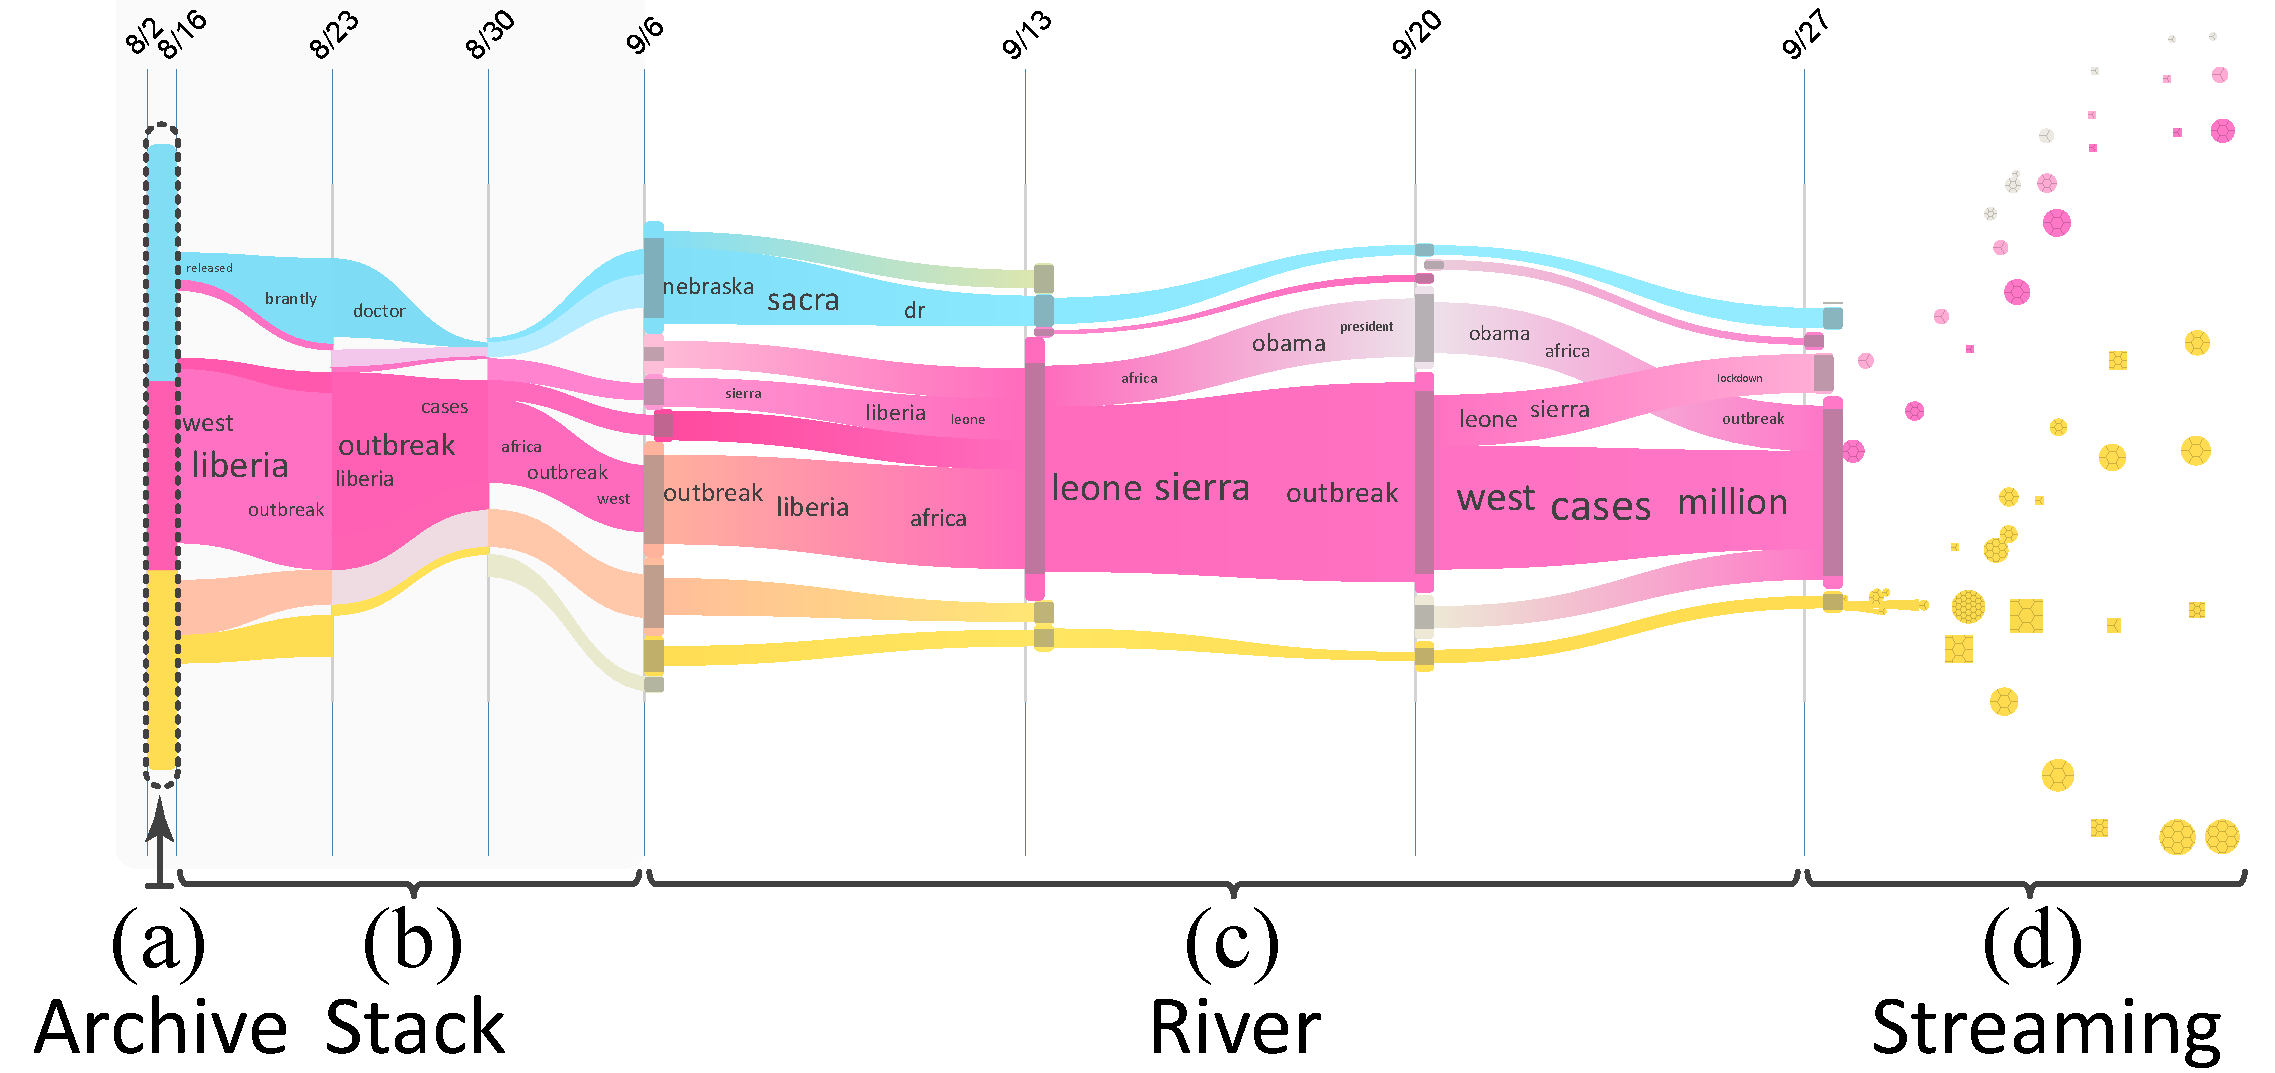
\includegraphics[width=\columnwidth]{fig/fourAreas}
	\vspace{-4mm}
	\caption{The visualization is divided into four areas: (a) archive; (b) stack; (c) river; (d) streaming.}
    %\vspace{-5mm}
	\label{fig:fourAreas}
\end{figure}

\subsection{Visualization Overview}

%Based on the guidelines described in Sec.~\ref{sec:rationale}, we design the \emph{\normalsize TopicStream} visualization (Fig.~\ref{fig:fourAreas}).
Based on the guidelines described in Sec.~\ref{sec:rationale}, we \dc{designed} the \emph{\normalsize TopicStream} visualization (Fig.~\ref{fig:fourAreas}).
%We design the \emph{\normalsize TopicStream} visualization, which is shown in Fig.~\ref{fig:fourAreas}, \kg{based on the guidelines described in Sec.~\ref{sec:rationale}, }.
The \emph{\normalsize x}-axis represents time.
The cut nodes are visualized as vertical bars at the corresponding time step.
The evolutionary relationship between cut nodes is represented by the stripes between the corresponding vertical bars.
%The flowing dots on the right side represents the newly arrived documents that are currently streaming in.
The flowing dots on the right side \kg{represent} the newly arrived documents that are currently streaming in.
%The different colors encodes different topics.
The different colors encode \kg{various} topics.\looseness=-1

%The core interest of our visualization is to help users track the dynamic characteristics of text streams.
The core \dc{intent} of our visualization is to help users track the dynamic characteristics of text streams.
%Every detail in our design is carefully crafted to cater for this purpose.
%Every detail in our design is carefully crafted to cater \kg{to} this purpose.
Every detail in our design \dc{was} carefully crafted to cater \kg{to} this purpose.
%For example, sedimentation animation is used to merge newly arrived documents into the dominant center of the visualization (\textbf{R2}).
%For example, sedimentation animation is used to merge newly arrived documents \kg{in} the dominant center of visualization (\textbf{R2}).
For example, sedimentation animation is used to merge newly arrived documents \kg{in} the dominant center of \dc{the} visualization (\textbf{\normalsize R2}).
% and gradually merge them with exiting topics.
%When more and more documents arrive, topic bars will gradually move to the other side of the display and leave more space for new topics (\textbf{R1}).
\kg{As the number of arriving documents increases}, topic bars gradually move to the other side of the display and leave \kg{a} space for new topics (\textbf{\normalsize R1}).
%With this mechanisms, users can more focus on the latest development of topics and find interesting patterns to conduct further analysis.
%With \kg{such} mechanisms, users can focus on the latest development of topics and \kg{identify} interesting patterns to conduct further analysis.
With \kg{such} mechanisms, users can focus on the latest development of topics and \kg{identify} interesting patterns to conduct further analysis.
%Specifically, the visualization consists of four regions (Fig.~\ref{fig:fourAreas}, \textbf{R1}):
\kg{In particular,} the visualization consists of four regions (Fig.~\ref{fig:fourAreas}, \textbf{\normalsize R1}):\looseness=-1
\begin{enumerate}
%\item \textbf{Stack}, which is next to the archive region and contains the older topics and documents that are compressed together due to the limited screen space;

\item \textbf{\normalsize Streaming}, which is on the rightmost side of \dc{the} visualization\kg{,} consists of newly streamed-in documents (e.g., the time period after Sep. 27  in Fig.~\ref{fig:fourAreas}(d)).

\item \textbf{\normalsize River}, which is the dominant region of \dc{the} visualization\kg{,} consists of recent topics \kg{along with} their splitting and merging relationships (e.g., Sep. 6 - 27 in Fig.~\ref{fig:fourAreas}(c)).

\item \textbf{\normalsize Stack}, which is to the left of the river region\kg{,} contains older topics and documents (e.g., Aug. 16 - Sep. 6 in Fig.~\ref{fig:fourAreas}(b)).
To reduce the visual complexity caused by the splitting and merging relationships, this region removes splitting/merging branches and only displays the mainstream of each topic.
Since users want to keep track of how the topics in this region connected with the topics in the river region, the white spaces between the topic stripes are not removed.
The width of each time step in this region is smaller than that in the river region to save space.\looseness=-1

\item \textbf{\normalsize Archive}, which is on the leftmost side, contains the oldest topics and documents (e.g., Aug. 2 - 16 in Fig.~\ref{fig:fourAreas}(a)).
 %that are compressed together \kg{because of} the limited screen space.
%Although the stacked region can save a certain amount of space, it is still cluttered for a text stream with tens or even hundreds of time steps.
Although the stacked region can \docpr{reduce the} amount of space \docpr{required}, it is still cluttered for a text stream with tens or even hundreds of time steps.
To solve this issue, we introduce the archive region,
which uses a stacked bar (Fig.~\ref{fig:fourAreas}(a)) to represent documents whose times are \emph{\normalsize k} time steps earlier than the newly streamed-in ones.
In \emph{\normalsize TopicStream}, \emph{\normalsize k} is specified by the user.
For example, \emph{\normalsize k} is set to 8 in the example of Fig.~\ref{fig:fourAreas}.
%To allocate more space for the recent documents as well as keep historical information in context, a bar region is used to encode documents whose times are \emph{\normalsize k} time steps earlier than the recent ones.
%In \emph{\normalsize TopicStream}, \emph{\normalsize k} is set by the user.
%For example, in the Ebola dataset, \emph{\normalsize k} is set to 7 by the expert.
To save space, the width of the bar is fixed no matter how many documents are archived.
Each bar item represents a topic.
Its height represents the average number of documents of each time step that belongs to this region.
%When a user examines the historically relevant documents, this region will be expanded as a stack graph with packed documents (Fig.~\ref{fig:dochighlight}).

%\item \textbf{River}, which is the dominant region of the visualization and consists of the recent topics and their splitting and merging relationships;
%\item \textbf{River}, which is the dominant region of visualization\kg{,} consists of recent topics \kg{along with} their splitting and merging relationships; \kg{and}

%\item \textbf{Streaming}, which is on the rightmost side of the visualization and consists of the newly streamed-in documents.
%\item \textbf{Streaming}, which is on the rightmost side of visualization\kg{,} consists of newly streamed-in documents.

\end{enumerate}
%The visual design of the archive and stack regions are quite straightforward. In this section, we will introduce the visual design of the river and streaming regions in detail.
%As described above, the archive and stack regions employ a bar and a stacked graph to show the corresponding topics.
%As described above, the visualization designs of a bar and a stacked graph are quite straightforward.
As described above, the visualization designs \docpr{for} a bar and a stacked graph are quite straightforward.
%We then introduce the visualization \kg{designs} of the river and streaming regions in detail.
We \docpr{will next} introduce the visualization \kg{designs} of the river and streaming regions in detail.

%The visual encodings used in our system are illustrated below.

\subsection{Visualization Design}
%\subsubsection{Tree Cut as River}
\subsubsection{Tree Cut as \kg{a} River}

\noindent\textbf{\normalsize Visual Encoding.}
%As in~\cite{cui2014}, each cut node is represented by a vertical bar (topic bar).
Each cut node is represented by a vertical bar (topic bar) \kg{similar to that presented in~\cite{cui2014}.}
The tree depth of a cut node is represented by the horizontal offset to the time step.
%The deeper a node in the tree, the further the corresponding topic bar moved to the right.
\kg{When} a node in the tree \kg{is deep}, the corresponding topic bar \kg{moves} to the right.

%The number of documents contained by a topic node is represented by the height of the topic bar.
The number of documents contained \kg{in} a topic node is represented by the height of the topic bar.
The width of the colored stripe between two topic bars indicates the number of document pairs between the two bars.
For example, the left width of the stripe represents the portion of documents mapped to the documents in the right topic bar.
%The dark region in the middle of a topic bar represents the portion of documents mapped to the documents both in the previous and next topic trees.
The dark region in the middle of a topic bar represents the portion of documents mapped to the documents both in the previous and \kg{the} next topic trees (Fig.~\ref{fig:fourAreas}).


\noindent\textbf{\normalsize Layout.}
%The basic representation of the visualization is a directed acyclic graph (DAG).
The basic representation of the visualization is a directed acyclic graph (DAG).
%A node represents a topic, and an edge between nodes encodes the evolutionary relationships between topics with mapping.
A node represents a topic and an edge between nodes encodes the evolutionary relationships between topics with mapping.
%When a new batch of documents are processed, we first run the DAG layout algorithm to find an optimal order for the new topic nodes.
When a new batch of documents \kg{is} processed, we first run the DAG layout algorithm to \kg{determine} an optimal order for the new topic nodes.
Once the topological structure is computed,  a force model is built to generate the sedimentation animation and merge new documents with existing topic bars.

\begin{figure}[t]
  \centering
  % \rule{2cm}{2cm}
 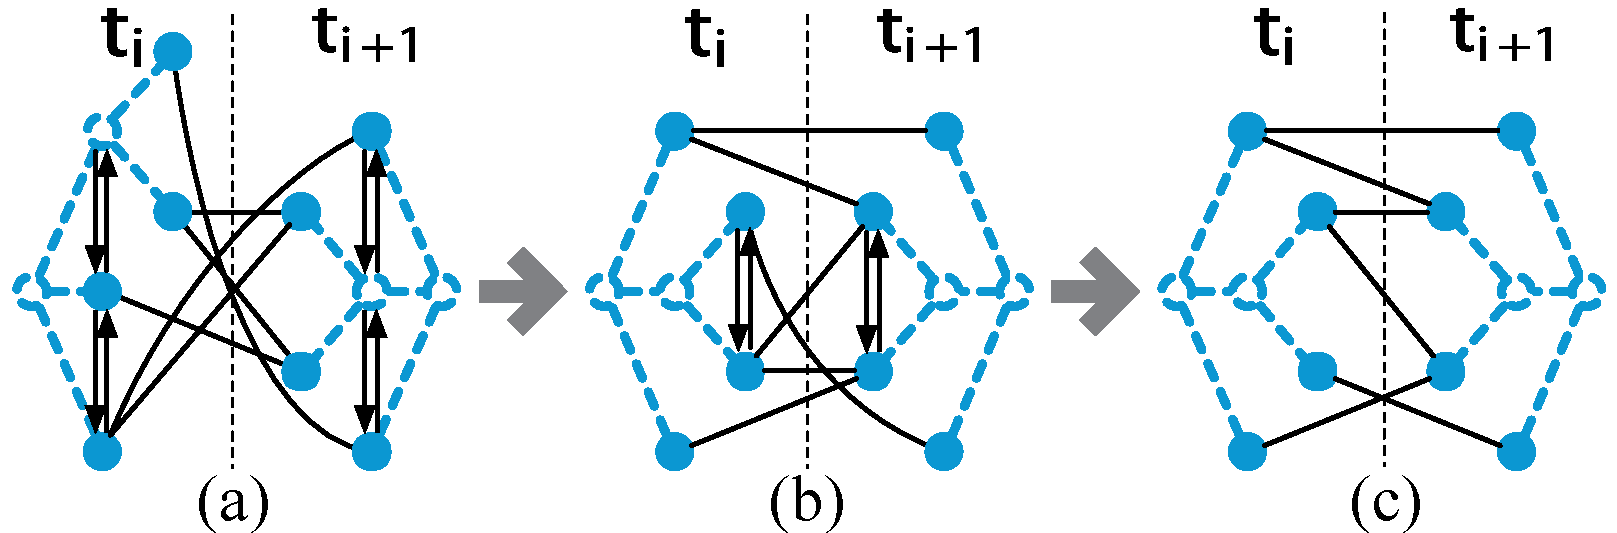
\includegraphics[width=\columnwidth]{fig/reorder}
 \vspace{-3mm}
  \caption{
%  \small
%  Example of reordering in levels: (a) reorder level one; (b) reorder level two; (c) result.
Reordering example: (a) reorder level one; (b) reorder level two; (c) result.
}
  \label{fig:reorder}
  \vspace{-1mm}
\end{figure}

\begin{figure}[t]
  \centering
  % \rule{2cm}{2cm}
 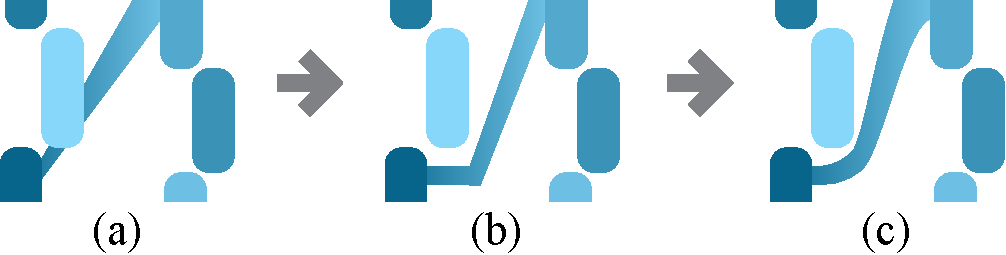
\includegraphics[width=3in]{fig/route}
 %\vspace{-3mm}
  \caption{
  %Example of edge routing: (a) the stripe is hidden by the topic bar; (b) two more intermediate points are added; (c) a B\'{e}zier curve is utilized to improve the visual quality.
  Example of edge routing: (a) the stripe is hidden by the topic bar; (b) two intermediate points are added; (c) a B\'{e}zier curve is utilized to improve visual quality.
  }
  \label{fig:route}
  \vspace{-5mm}
\end{figure}


%\subsubsection{Reordering and Edge Routing}

%To generate a legible layout and better illustrate the evolving patterns, we first reorder the cut nodes at each time point to minimize edge crossings between neighboring time points, then route edges to avoid overlapping between nodes and edges, and finally representative documents on a selected stripe.
We \kg{initially} reorder the cut nodes at each time step to minimize edge crossings between neighboring time steps \kg{and generate a legible layout that illustrates the evolving patterns.} \kg{Edges are then routed} to avoid overlapping between nodes and edges. \kg{Finally}, representative documents \kg{are packed} on a selected stripe.

%\emph{\normalsize Reordering.} Sugiyama's heuristics~\cite{Sugiyama1981}, a well-known DAG layout algorithm, is employed to reorder the nodes at each time to minimize edge crossings.
\emph{\normalsize Reordering.} Sugiyama's heuristics~\cite{Sugiyama1981}, \kg{which is} a well-known DAG layout algorithm, is employed to reorder the nodes at each time step to minimize edge crossings.
%However, if we directly run the algorithm without constraints, the sibling nodes may be separated by other nodes.
However, if we directly run the algorithm without constraints, sibling nodes \kg{can} be separated by other nodes.
%To ensure that the sibling nodes stay together, we implement Sugiyama's heuristics from the top to the lowest level of the tree at each time.
%We implement Sugiyama's heuristics from \kg{highest} to the lowest \kg{levels} of the tree at each time \kg{to ensure that the sibling nodes stay together}
We implement Sugiyama's heuristics from \dc{the} \kg{highest} to the lowest \kg{levels} of the tree at each time \kg{to ensure that the sibling nodes stay together}\dc{.}
%The sibling nodes with the same parent are regarded as a compound node.
%At each level, we first reorder the sibling nodes inside each compound node, then sort the compound nodes accordingly.
Fig.~\ref{fig:reorder} provides an example generated by the reordering algorithm.

%\emph{\normalsize Edge Routing.} The stripes and topic bars may overlap because the topic nodes are offset to encode their depth (Fig.~\ref{fig:route}(a)).
\emph{\normalsize Edge Routing.} \kg{Stripes} and topic bars \kg{can} overlap because topic nodes are offset to encode their depth (Fig.~\ref{fig:route}(a)).
We employ the edge routing technique~\cite{Cui2008} to solve this problem.
Two additional intermediate points are introduced for each overlapping part to route the stripe.
%Two additional intermediate points are introduced for each overlapping \docpr{section} to route the stripe and avoid overlapping.
The B\'{e}zier curve is utilized to help users follow the striped path (Fig.~\ref{fig:route}).

\begin{figure}[t ]
  \centering
  % \rule{2cm}{2cm}
  \vspace{-3mm}
 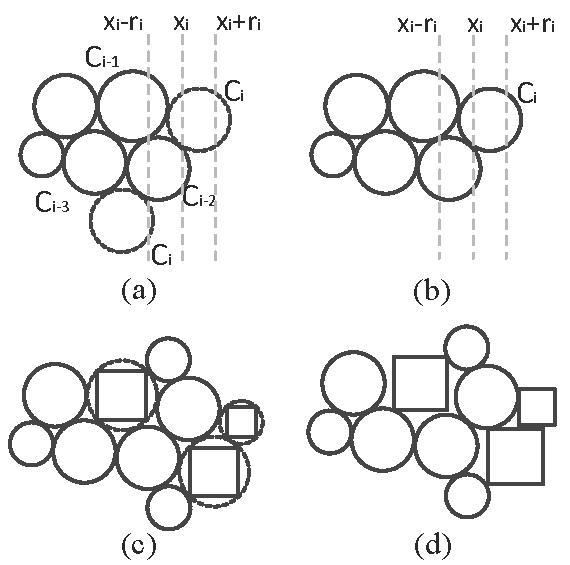
\includegraphics[width=0.7\linewidth]{fig/packing}
 \vspace{-1mm}
  \caption{
  %Illustration of the packing algorithm: (a) find possible placement positions of $C_i$; (b)set the position closest to ($x_i$, 0) as the placement position; (c) replace some circles by the corresponding rectangles; (d) reduce the gap with the size constraint and derive the final packing result.
  Illustration of the packing algorithm:
  (a) \kg{finding} possible placement positions of $C_i$;
  (b) \kg{setting} the position closest to ($x_i$, 0) as the placement position;
  (c) \kg{replacing several} circles \kg{with} the corresponding squares;
  %(d) \kg{reducing} the gap with the size constraint and \kg{deriving} the final packing result.\looseness=-1
  (d) \kg{reducing} the gap with the size \docpr{constraints} and \kg{deriving} the final packing result.\looseness=-1
  }
  \label{fig:packing}
  \vspace{-3mm}
\end{figure}

\begin{figure}[b]
  \centering
  \vspace{-3mm}
 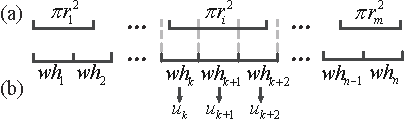
\includegraphics[width=2.6in]{fig/packposition3}
  \caption{
  %Derivation of the initial \emph{x} position.
  \kg{Deriving} the initial \emph{x} position:
  (a) align all the circles on a straight line based on their areas;
  (b) align all the stripe segments on a straight line based on their areas.
  %The dotted vertical lines indicate the overlapping relationship the area of the circle and that of the segmented stripes.
  The dotted vertical lines indicate the overlapping relationship \docpr{between} the area of the circle and that of the segmented stripes.
%Based on the relationship, $\normalsize x_i$ is approximated by $\normalsize average(u_k, u_{k+1}, u_{k+2})$.
  Based on \docpr{this} relationship, $\normalsize x_i$ is approximated \docpr{as an} $\normalsize average(u_k, u_{k+1}, u_{k+2})$.
  }
  \label{fig:xvalue}
\end{figure}

%\begin{figure}[t]
%  \centering
%  % \rule{2cm}{2cm}
%%  \vspace{-3mm}
% 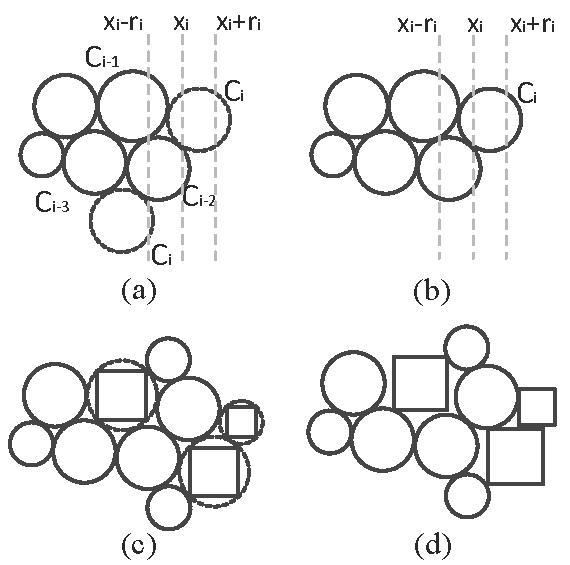
\includegraphics[width=0.7\linewidth]{fig/packing}
% \vspace{-2mm}
%  \caption{
%  %Illustration of the packing algorithm: (a) find possible placement positions of $C_i$; (b)set the position closest to ($x_i$, 0) as the placement position; (c) replace some circles by the corresponding rectangles; (d) reduce the gap with the size constraint and derive the final packing result.
%  Illustration of the packing algorithm: (a) \kg{finding} possible placement positions of $C_i$; (b) \kg{setting} the position closest to ($x_i$, 0) as the placement position; (c) \kg{replacing several} circles \kg{with} the corresponding rectangles; (d) \kg{reducing} the gap with the size constraint and \kg{deriving} the final packing result.}
%  \label{fig:packing}
%  \vspace{-3mm}
%\end{figure}



%\emph{\normalsize Packing}. To help users understand and compare the relationships between documents, including the coming order and similarity relationships, we pack them on the topic stripe (\textbf{R3}).
\emph{\normalsize Packing}. We pack \kg{the documents} on the topic stripe %(\textbf{\normalsize R3}) \kg{to help users understand and compare their relationships, including incoming order and similarity relationships.}
(\textbf{\normalsize R3}) \kg{to help users understand and compare their relationships, \docpr{including the incoming} order and similarity relationships.}
%In our visualization, each news article cluster is represented by a circle, while each Twitter cluster is represented by a rectangle.
Each news article is represented by a circle \kg{in our visualization}, \kg{whereas} each tweet is represented by a square.
%For simplicity, each rectangle is approximately represented by a circle whose center is that of the rectangle and whose radius is $\beta\cdot\sqrt{2}a$.
For \dc{the sake of} simplicity, each square is approximately represented by a circle whose center is \dc{the same as} the square\dc{'s} and whose radius is $\beta\cdot\sqrt{2}b$.
%Each rectangle is approximately represented by a circle whose center is \kg{that} of the rectangle and whose radius is $\beta\cdot\sqrt{2}a$ \kg{for simplicity}.
%Here $a$ is the side length of the rectangle and $\beta$ ($1\leq\beta\leq1/\sqrt{2}$) is a parameter to balance the intersection and gap between the elements (e.g., circles and rectangles) in the final packing result.
%$a$ is the side length of the rectangle and $\beta$ ($1\leq\beta\leq1/\sqrt{2}$) is a parameter \kg{that balances} intersection and gap\kg{s} between elements (e.g., circles and rectangles) in the final packing result.
%$b$ is the side length of the rectangle and $\beta$ ($1\leq\beta\leq1/\sqrt{2}$) is a parameter \kg{that balances} \dc{the} intersection and gap\kg{s} between elements (e.g., circles and rectangles) in the final packing result.
$\normalsize b$ is the side length of the square and $\beta$ ($1/\sqrt{2}\leq\beta\leq1$) is a parameter \kg{that balances} \dc{the} intersection and gap\kg{s} between elements (e.g., circles and squares) in the final packing result.
%The larger $\beta$ is, the more gap might be.
The larger $\beta$ is, the \dc{larger the} gap might be.
%This transformation preserves the area enclosed by the boundary.
%With this approximation, the packing problem is formulated as a circle packing problem.
The packing problem is formulated as a circle packing problem \kg{using this approximation}.
%We then employ a front-chain-based circle packing algorithm as in~\cite{Wang2006visualization,ZhaoTVCG2014} to tightly pack circles on the selected stripe.
%We then employ a front-chain-based circle packing algorithm as in~\cite{Wang2006visualization,ZhaoTVCG2014} to pack circles \kg{tightly} on the selected stripe.
We then employ a front-chain-based circle packing \docpr{algorithm, as in~\cite{Wang2006visualization,ZhaoTVCG2014}, to} pack circles \kg{tightly} on the selected stripe.
%Fig.~\ref{fig:packing} illustrate the basic idea of this packing algorithm.
Fig.~\ref{fig:packing} illustrate\kg{s} the basic idea of this packing algorithm.
%Fig.~\ref{fig:packing} illustrate\kg{s} the basic \docpr{concept} of this packing algorithm.

%Compared with the packing problem described in~\cite{ZhaoTVCG2014}, ours does not provide the initial \emph{x}-coordinate for each circle.
Compared with the packing problem described in~\cite{ZhaoTVCG2014}, our \kg{problem} does not provide the initial \emph{x} coordinate for each circle.
%In our packing problem, only the coming order of each circle is provided.
Only the incoming order of each circle is provided in our packing problem.
%Thus, we need to derive the initial \emph{x}-coordinate based on the order of circles.
Thus, we \kg{have} to derive the initial \emph{x} coordinate based on the order of \kg{the} circles.
%The basic idea is to find an approximate placement position of each circle, which is achieved by approximately mapping its area to the area of the segmented stripes in ascending order.
The basic idea is to \kg{determine} an approximate placement position \kg{for} each circle, which is achieved by approximately mapping its area to the area of the segmented stripes.
%Then the averaged x-coordinates of the corresponding segmented stripes is used to approximate the initial x-coordinate of the circle.
%The averaged \emph{x} coordinates of the corresponding segmented stripes is \kg{then} used to approximate the initial \emph{x} coordinate of the circle.
The average \dc{of the} \emph{x} coordinates of the corresponding segmented stripes is \kg{then} used to approximate the initial \emph{x} coordinate of the circle.
%Specifically, we align all the circles on a straight line based on their areas (Fig.~\ref{fig:xvalue}(a)).
\kg{In particular}, we align all the circles on a straight line based on their areas (Fig.~\ref{fig:xvalue}(a)).
The area of circle $C_i$ is $\pi{r_i}^2$.
%For simplicity, we denote it by ${r_i}^2$.
%Next, we divide the stripe into \emph{\normalsize n} uniform segments along its \emph{x}-axis.
We \kg{then} divide the stripe into \emph{\normalsize n} uniform segments along its \emph{x}-axis.
The height of the \emph{\normalsize k}-th segment is denoted as $h_k$ and its area is $wh_k$,
%Here $w$ is the width of each segment along the \emph{x}-axis.
\kg{where} $w$ is the width of each segment along the \emph{x}-axis.
All these segments are also aligned on a straight line based on their areas (Fig.~\ref{fig:xvalue}(b)).
%As shown in Fig.~\ref{fig:xvalue}, with these two straight lines, the overlapping relationship between the area of the circle and that of the segmented stripes can be discovered.
Fig.~\ref{fig:xvalue} \kg{shows that} the overlapping relationship between the area of the circle and that of the segmented stripes can be \kg{determined using two straight lines}.
%For example, in this figure, the initial $x_i$ is approximated by $average(x_k, x_{k+1}, x_{k+2})$.
%For example, the initial $x_i$ in this figure is approximated by $average(x_k, x_{k+1}, x_{k+2})$.
For example, the initial $x_i$ of circle \emph{\normalsize i} in this figure is approximated by $\normalsize average(u_k, u_{k+1}, u_{k+2})$.
Here $u_k$ is the \emph{x} coordinate of the center of \emph{\normalsize k}-th segment.

\noindent \textbf{\normalsize Interaction}.
%In addition to the interactions described in~\cite{cui2014}, such as details on demand, collapsing/expanding time points, splitting/merging topic bars, and changing focus, we also provide the following interactions to explore the complex evolutionary clustering results from multiple perspectives.
%We also provide the following interactions to explore the complex evolutionary clustering results from multiple perspectives \kg{aside from the interactions described in~\cite{cui2014} (e.g. details on demand, collapsing/expanding time points, splitting/merging topic bars, and changing focus).}
%We also provide the following interactions to explore the complex evolutionary clustering results from multiple perspectives \kg{aside from the interactions described in~\cite{cui2014} (e.g. details on demand, collapsing/expanding time steps, splitting/merging topic bars, and changing focus).}
We also provide the following interactions to explore the complex evolutionary clustering results from multiple perspectives \kg{\docpr{in addition to} the interactions described in~\cite{cui2014} (e.g. details on demand, collapsing/expanding time steps, splitting/merging topic bars, and changing focus).}

\emph{\normalsize Document Query}.
%Once the tokens have transformed into a colored stripe, we adopt voronoi treemap~\cite{} to encode the containing documents within the color stripe for further query and analysis.
Once the documents \kg{are} transformed into a colored stripe, we adopt \kg{circle packing} to encode the documents \kg{contained} within the color stripe for further query and analysis.
%In the example shown in  Fig.~\ref{fig:vtreemap}, users can click the stripe and turn it into a treemap, in which thicker borders indicate tokens while the thin borders indicate documents contained by each token.
%The example in  Fig.~\ref{fig:vtreemap} \kg{shows that} users can click the stripe and turn it into a circle/rectangle packing, in which a circle represents a news article \kg{whereas} the rectangle encodes a tweet.
The example in  Fig.~\ref{fig:vtreemap} \dc{shows how} users can click the stripe and turn it into a circle/square packing, in which a circle represents a news article \dc{and a} square encodes a tweet.
%From this figure, we can easily see the number of tokens that sediment to this topic and compare their relative size.
%\kg{This} figure \kg{shows} the number of tokens that sediment \kg{into} this topic and compare\kg{s} their relative size\kg{s}.
%Once the packing result is displayed, users can manually click one or more document to examine their content in detail.
Once the packing result is displayed, users can manually click one or more \dc{documents} to examine \dc{the} content in detail.

\emph{\normalsize Visual Comparison}.
%By leveraging circle packing algorithm, we allow users to compare the relationships among different time points.
%We allow users to compare the relationships among different time points \kg{by leveraging circle packing algorithm.}
We allow users to compare the relationships among different time steps by leveraging \dc{a} circle packing algorithm.
%For example, users can compare the incoming order and similarity relationships in Fig.~\ref{fig:ebola}(a) and in Fig.~\ref{fig:ebola}(b).
%For example, users can compare the incoming order and similarity relationships Fig.~\ref{fig:ebola}(a) and Fig.~\ref{fig:ebola}(b).
For example, users can compare the incoming order and similarity relationships\docpr{, as shown in} Fig.~\ref{fig:ebola}(a).
%One of our experts, professor P2 commented, ``Comparing the incoming order of documents help me easily discover who talk a topic first (set the agenda) and who follows immediately.
%One of our experts, P2, commented \kg{that}, ``Comparing the incoming order of documents \dc{helps} me easily discover who \kg{talked about} a topic first (\kg{that is, who} set the agenda) and who follow\kg{ed} immediately.
One of our experts, P2, commented \kg{that}, ``Comparing the incoming order of documents \dc{helps} me easily discover who \kg{talked about} a topic first (\kg{that is, who} set the agenda) and who \docpr{immediately follow\kg{ed}}.
%This \kg{feature} is useful \kg{to study} agenda setting in my field.''
This \kg{feature} \dc{can help me} \kg{study} agenda setting in my field.''

\subsubsection{Streaming Document as Sedimentation}

%\begin{figure}[t]
%  \centering
% 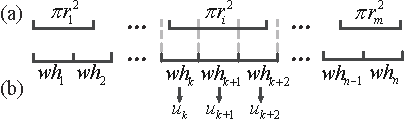
\includegraphics[width=2.6in]{fig/packposition3}
%  \caption{
%  %Derivation of the initial \emph{x} position.
%  \kg{Deriving} the initial \emph{x} position: (a) align all the circles on a straight line based on their areas; (b) align all the stripe segments on a straight line based on their areas. The dotted vertical lines indicate the overlapping relationship the area of the
%circle and that of the segmented stripes. Based on the relationship, $\normalsize x_i$ is approximated by $\normalsize average(u_k, u_{k+1}, u_{k+2})$.
%  }
% \vspace{-3mm}
%  \label{fig:xvalue}
%\end{figure}

\begin{figure}[b]
	\vspace{-3mm}
	\centering
	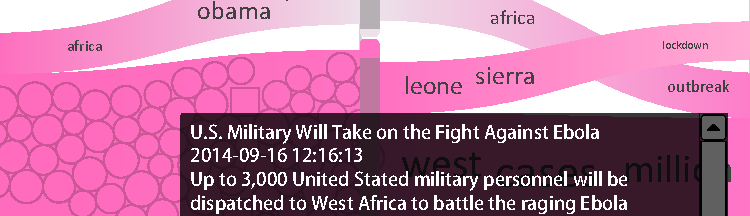
\includegraphics[width=\columnwidth]{fig/vtreemap}
	\vspace{-5mm}
	\caption{
	%Encode documents after sedimentation as a \kg{circle/square packing}.
	Encode documents after sedimentation \docpr{as \kg{circle/square packing}}.
	}
	\label{fig:vtreemap}
%	\vspace{-3mm}
\end{figure}


\noindent \textbf{\normalsize Visual Encoding}.
%Inspired by visual sedimentation~\cite{Huron2013visual}, we use the river sedimentation metaphor to encode the process of newly arrived text documents merging with existing topics (\textbf{R2}).
Inspired by visual sedimentation~\cite{Huron2013visual}, we use the river sedimentation metaphor to encode the process of newly arrived text documents \kg{that merge} with existing topics (\textbf{\normalsize R2}).
To quicken the sedimentation process of a high-volume text stream, a set of document clusters are derived from the incoming documents by using k-means clustering.
A token is a visual mark representing a document cluster.
%The generation process of the sedimentation metaphor consists four steps:
The generation process of the sedimentation metaphor consists \dc{of} four steps:

\emph{\normalsize Entrance}.
%Newly arrived documents are represented as circular or rectangular tokens (Fig.~\ref{fig:fourAreas}) and flying into the view from the right hand side.
Newly arrived documents are represented as circular or rectangular tokens (Fig.~\ref{fig:fourAreas}) \kg{that come} into view from the right side.
%To handle the scalability issue, documents of similar content are clustered into one token, the size of which indicates the document number.
Documents \kg{with} similar content are clustered into one token, the size of which indicates the \kg{number of} documents, \kg{to handle the scalability issue}.
The color of each token encodes the topic that it contains.

\emph{\normalsize Suspension}.
%Each token will fly towards (from right to left) the corresponding topic bars of the latest time point.
Each token \kg{moves toward} (from right to left) the corresponding topic bars of the latest time step.
%During the movement, the sizes of tokens will decrease gradually.
%\kg{Token sizes} decrease gradually \kg{during the movement}.
Token \dc{size} \dc{decreases} gradually \kg{during the movement}.

\emph{\normalsize Accumulation} and \emph{\normalsize decay}.
%Once tokens touch the corresponding topic bars or other tokens that have already settled, they will stop moving and begin to shrink (decay).
\kg{The tokens} will stop moving and start \kg{to} decay \kg{once they touch the corresponding topic bars or other tokens that have already settled.}
%The settled tokens will continue to .
The settled tokens continue to shrink and merge \kg{with} existing topics.

\emph{\normalsize Aggradation}.
%When the settled tokens resolve, the colored stripes continue to grow and indicates the latest development of news topics.
The colored stripes continue to grow and \kg{indicate} the latest development of topics \kg{when the settled tokens are resolved}.

%Once a batch of news documents (e.g., for a day) are all sedimented, corresponding topic bars will appear, and push older topic bars to the left hand side.
%Once a batch of news documents (e.g., for a day) are all sedimented, \kg{the} corresponding topic bars appear and push older topic bars to the hand side.
%Once a batch of documents (e.g., for a day) are all sedimented, \kg{the} corresponding topic bars appear and push older topic bars to the \dc{left-hand} side.
Once a batch of documents (e.g., for a day) \docpr{are sedimented}, \kg{the} corresponding topic bars appear and push older topic bars to the \dc{left-hand} side.
%The achieve and the stack regions will change accordingly.
The archive and stack regions \kg{then} change accordingly.

\begin{figure}[t]
	\centering
	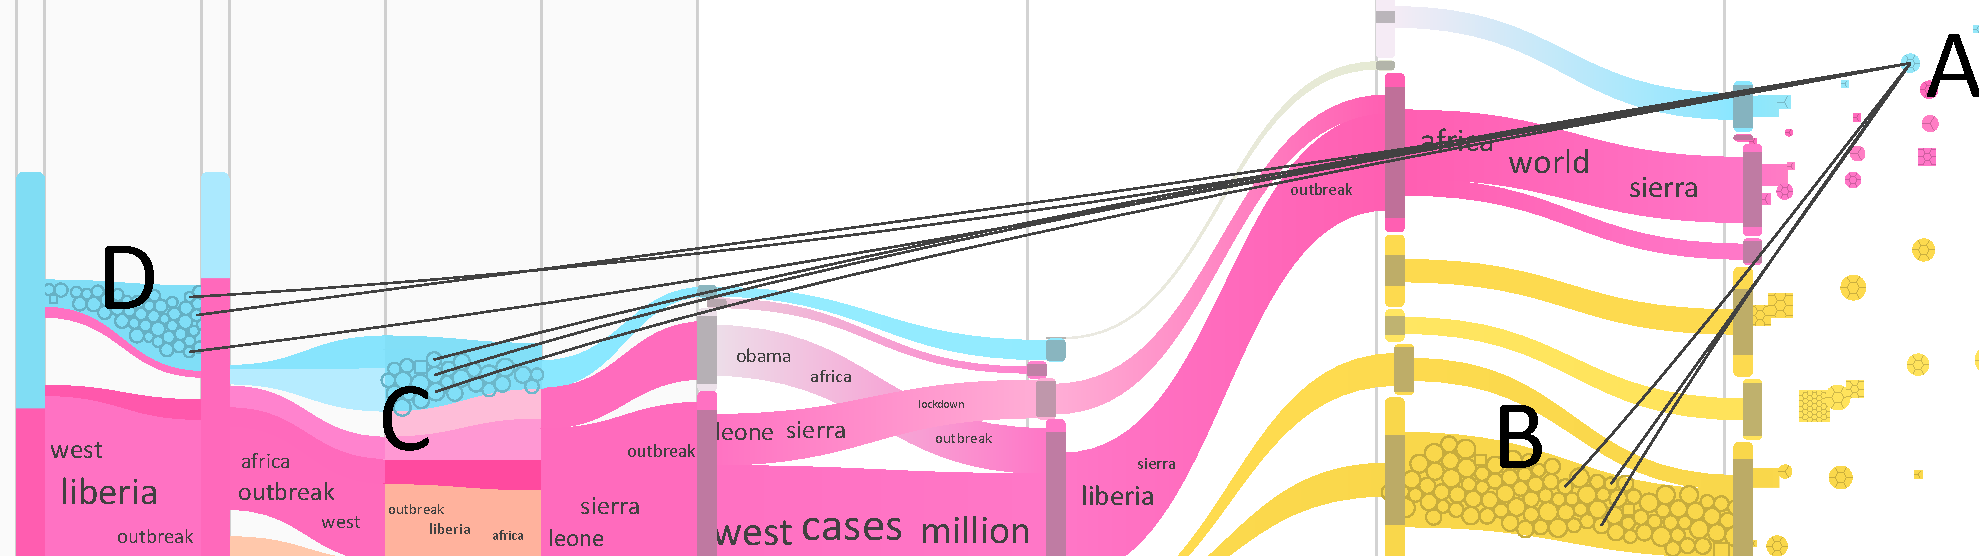
\includegraphics[width=\columnwidth]{fig/docHighlight}
	\vspace{-4mm}
%	\caption{Relevant documents of cluster A are highlighted in both the river (B) and the archive (C) regions.\looseness=-1}
	\caption{
	%Relevant documents of cluster A are highlighted in both the river (B)\xiting{, the stack (C),} and the archive (\xiting{D}) regions.\looseness=-1
	Relevant documents of cluster A are highlighted \docpr{in the} river (B)\xiting{, the stack (C),} and the archive (\xiting{D}) regions.\looseness=-1
	}
\vspace{-5mm}
	\label{fig:dochighlight}
\end{figure}

\noindent \textbf{\normalsize Layout}.
%During the sedimentation process, each token is given a region based on the topological structure in the ``reordering and edge routing'' step.
Each token is \kg{assigned to} a region based on the topological structure in the ``reordering and edge routing'' step \kg{during the sedimentation process.}
%The token can only move within the given region, and cannot cross the border.
%The token can only move within the \kg{assigned to} region, and cannot cross the border.
The token can only move within the \dc{assigned region} and cannot cross the border.
%The moving speed of the token is controlled by two forces: 1) a universal gravity force and 2) an attractive force between the moving token and the tokens that are already sedimented.
%The moving speed of the token is controlled by two forces: 1) a universal gravity force and 2) an attractive force between the token and the \kg{sedimented} tokens.
The \dc{speed} of the token is controlled by two forces: 1) a universal gravity force and 2) an attractive force between the token and the \kg{sedimented} tokens.
%The gravity force provides each token a constant acceleration from right to left.
The gravity force provides each token \kg{with} constant acceleration from right to left.
%The attractive force ensures that similar documents will sediment close to each other.
The attractive force ensures that similar documents will sediment close to \kg{one another.}
Therefore, the total acceleration $a_k$ for a moving token $k$ is defined as
$$a_k=g+\sum_is_{ik}*{n_i}/{||p_i-p_k||^2},$$
%where $g$ is the constant gravity acceleration, $p_i$ is the location of token $i$ that is already sedimented, $p_k$ is the location of token $k$, $m_i$ is the number of documents in token $i$, and $s_{ik}$ is the content similarity between token $i$ and $k$.
where $g$ is the constant gravity acceleration, $p_i$ is the location of \kg{sedimented} token $i$, $p_k$ is the location of token $k$, $n_i$ is the number of documents in token $i$, and $s_{ik}$ is the content similarity between token\kg{s} $i$ and $k$.


%\noindent \textbf{\normalsize Interaction}
\noindent \textbf{\normalsize \xiting{Interaction.}}
%The sedimentation visualization also to allow users to interactively examine the content of new coming documents and compare them with the older documents.
%The sedimentation visualization also allow\kg{s} users to examine the content of \kg{incoming} documents \kg{interactively} and compare them with older documents.
The sedimentation visualization also allow\kg{s} users to examine the content of \docpr{the} \kg{incoming} documents \kg{interactively} and compare them with older documents.

\emph{\normalsize Document Link}.
%In many text stream analysis tasks, it is desired to quickly find related documents covering a long range of time period.
In many text stream analysis tasks, it is \dc{desirable} to quickly find related documents covering a long \dc{time} period.
%\kg{Finding} related documents \kg{that rapidly cover} a long range of period \kg{is the objective of many text stream analyses}.
%In our system, document highlight is supported for this need.
Document link is supported for this \kg{requirement of our system}.
%Document link is \docpr{therefore supported by} our system.
%For example, users may first explore the content in the streaming region, and find a document of interest.
For example, users \kg{can initially} explore the content in the streaming region and find a document/cluster of interest.
%Then, our system will automatically use the word vector in the given document, and locate the most similar documents in all three regions (i.e., streaming, stack, and achieve).
Our system \kg{then} automatically use\kg{s} the word vector in the given document and locate\kg{s} the most similar documents in all three regions (i.e., streaming, stack, and archive).
%Once the related documents are located, containing treemap cells or circular tokens will be automatically highlighted and connections will be displayed for users to further exploration.
Once the related documents/clusters are located, the connections \kg{are} displayed for users to \kg{explore further}.

%An example of document highlight is shown in Fig.~\ref{fig:dochighlight},
An example of document \dc{link} is shown in Fig.~\ref{fig:dochighlight},
%where a user explores the relevant documents of a new coming twitter cluster (Fig.~\ref{fig:dochighlight}A).
\kg{in which} a user explores relevant documents \kg{from an incoming Twitter} cluster (Fig.~\ref{fig:dochighlight}A).
%Relevant documents are found in both the river region (Fig.~\ref{fig:dochighlight}B)\xiting{, the stack region (Fig.~\ref{fig:dochighlight}C),} and archive region (Fig.~\ref{fig:dochighlight}\xiting{D}).
%Relevant documents are found in the river (Fig.~\ref{fig:dochighlight}B), stack (Fig.~\ref{fig:dochighlight}C), archive (Fig.~\ref{fig:dochighlight}D) \kg{regions}.
Relevant documents are found in the river (Fig.~\ref{fig:dochighlight}B), stack (Fig.~\ref{fig:dochighlight}C), \dc{and} archive (Fig.~\ref{fig:dochighlight}D) \kg{regions}.
%To felicitate the examination of the highlighted documents, the archive region is expanded accordingly.
The archive region is expanded accordingly \kg{to facilitate the examination of the relevant documents.}

%In addition, users can also click on a token while it is still in the suspension step, related documents will also be displayed for further examination.
\kg{Users} can also click on a token while it is still in the suspension step.
%Then related documents \kg{are} displayed for further examination.
\dc{Related} documents \kg{are} \dc{then} displayed for further examination.


